% Options for packages loaded elsewhere
\PassOptionsToPackage{unicode}{hyperref}
\PassOptionsToPackage{hyphens}{url}
\PassOptionsToPackage{dvipsnames,svgnames,x11names}{xcolor}
%
\documentclass[
]{agujournal2019}

\usepackage{amsmath,amssymb}
\usepackage{iftex}
\ifPDFTeX
  \usepackage[T1]{fontenc}
  \usepackage[utf8]{inputenc}
  \usepackage{textcomp} % provide euro and other symbols
\else % if luatex or xetex
  \usepackage{unicode-math}
  \defaultfontfeatures{Scale=MatchLowercase}
  \defaultfontfeatures[\rmfamily]{Ligatures=TeX,Scale=1}
\fi
\usepackage{lmodern}
\ifPDFTeX\else  
    % xetex/luatex font selection
\fi
% Use upquote if available, for straight quotes in verbatim environments
\IfFileExists{upquote.sty}{\usepackage{upquote}}{}
\IfFileExists{microtype.sty}{% use microtype if available
  \usepackage[]{microtype}
  \UseMicrotypeSet[protrusion]{basicmath} % disable protrusion for tt fonts
}{}
\makeatletter
\@ifundefined{KOMAClassName}{% if non-KOMA class
  \IfFileExists{parskip.sty}{%
    \usepackage{parskip}
  }{% else
    \setlength{\parindent}{0pt}
    \setlength{\parskip}{6pt plus 2pt minus 1pt}}
}{% if KOMA class
  \KOMAoptions{parskip=half}}
\makeatother
\usepackage{xcolor}
\setlength{\emergencystretch}{3em} % prevent overfull lines
\setcounter{secnumdepth}{5}
% Make \paragraph and \subparagraph free-standing
\makeatletter
\ifx\paragraph\undefined\else
  \let\oldparagraph\paragraph
  \renewcommand{\paragraph}{
    \@ifstar
      \xxxParagraphStar
      \xxxParagraphNoStar
  }
  \newcommand{\xxxParagraphStar}[1]{\oldparagraph*{#1}\mbox{}}
  \newcommand{\xxxParagraphNoStar}[1]{\oldparagraph{#1}\mbox{}}
\fi
\ifx\subparagraph\undefined\else
  \let\oldsubparagraph\subparagraph
  \renewcommand{\subparagraph}{
    \@ifstar
      \xxxSubParagraphStar
      \xxxSubParagraphNoStar
  }
  \newcommand{\xxxSubParagraphStar}[1]{\oldsubparagraph*{#1}\mbox{}}
  \newcommand{\xxxSubParagraphNoStar}[1]{\oldsubparagraph{#1}\mbox{}}
\fi
\makeatother


\providecommand{\tightlist}{%
  \setlength{\itemsep}{0pt}\setlength{\parskip}{0pt}}\usepackage{longtable,booktabs,array}
\usepackage{calc} % for calculating minipage widths
% Correct order of tables after \paragraph or \subparagraph
\usepackage{etoolbox}
\makeatletter
\patchcmd\longtable{\par}{\if@noskipsec\mbox{}\fi\par}{}{}
\makeatother
% Allow footnotes in longtable head/foot
\IfFileExists{footnotehyper.sty}{\usepackage{footnotehyper}}{\usepackage{footnote}}
\makesavenoteenv{longtable}
\usepackage{graphicx}
\makeatletter
\def\maxwidth{\ifdim\Gin@nat@width>\linewidth\linewidth\else\Gin@nat@width\fi}
\def\maxheight{\ifdim\Gin@nat@height>\textheight\textheight\else\Gin@nat@height\fi}
\makeatother
% Scale images if necessary, so that they will not overflow the page
% margins by default, and it is still possible to overwrite the defaults
% using explicit options in \includegraphics[width, height, ...]{}
\setkeys{Gin}{width=\maxwidth,height=\maxheight,keepaspectratio}
% Set default figure placement to htbp
\makeatletter
\def\fps@figure{htbp}
\makeatother
% definitions for citeproc citations
\NewDocumentCommand\citeproctext{}{}
\NewDocumentCommand\citeproc{mm}{%
  \begingroup\def\citeproctext{#2}\cite{#1}\endgroup}
\makeatletter
 % allow citations to break across lines
 \let\@cite@ofmt\@firstofone
 % avoid brackets around text for \cite:
 \def\@biblabel#1{}
 \def\@cite#1#2{{#1\if@tempswa , #2\fi}}
\makeatother
\newlength{\cslhangindent}
\setlength{\cslhangindent}{1.5em}
\newlength{\csllabelwidth}
\setlength{\csllabelwidth}{3em}
\newenvironment{CSLReferences}[2] % #1 hanging-indent, #2 entry-spacing
 {\begin{list}{}{%
  \setlength{\itemindent}{0pt}
  \setlength{\leftmargin}{0pt}
  \setlength{\parsep}{0pt}
  % turn on hanging indent if param 1 is 1
  \ifodd #1
   \setlength{\leftmargin}{\cslhangindent}
   \setlength{\itemindent}{-1\cslhangindent}
  \fi
  % set entry spacing
  \setlength{\itemsep}{#2\baselineskip}}}
 {\end{list}}
\usepackage{calc}
\newcommand{\CSLBlock}[1]{\hfill\break\parbox[t]{\linewidth}{\strut\ignorespaces#1\strut}}
\newcommand{\CSLLeftMargin}[1]{\parbox[t]{\csllabelwidth}{\strut#1\strut}}
\newcommand{\CSLRightInline}[1]{\parbox[t]{\linewidth - \csllabelwidth}{\strut#1\strut}}
\newcommand{\CSLIndent}[1]{\hspace{\cslhangindent}#1}

\usepackage{url} %this package should fix any errors with URLs in refs.
\usepackage{lineno}
\usepackage[inline]{trackchanges} %for better track changes. finalnew option will compile document with changes incorporated.
\usepackage{soul}
\linenumbers
\makeatletter
\@ifpackageloaded{tcolorbox}{}{\usepackage[skins,breakable]{tcolorbox}}
\@ifpackageloaded{fontawesome5}{}{\usepackage{fontawesome5}}
\definecolor{quarto-callout-color}{HTML}{909090}
\definecolor{quarto-callout-note-color}{HTML}{0758E5}
\definecolor{quarto-callout-important-color}{HTML}{CC1914}
\definecolor{quarto-callout-warning-color}{HTML}{EB9113}
\definecolor{quarto-callout-tip-color}{HTML}{00A047}
\definecolor{quarto-callout-caution-color}{HTML}{FC5300}
\definecolor{quarto-callout-color-frame}{HTML}{acacac}
\definecolor{quarto-callout-note-color-frame}{HTML}{4582ec}
\definecolor{quarto-callout-important-color-frame}{HTML}{d9534f}
\definecolor{quarto-callout-warning-color-frame}{HTML}{f0ad4e}
\definecolor{quarto-callout-tip-color-frame}{HTML}{02b875}
\definecolor{quarto-callout-caution-color-frame}{HTML}{fd7e14}
\makeatother
\makeatletter
\@ifpackageloaded{caption}{}{\usepackage{caption}}
\AtBeginDocument{%
\ifdefined\contentsname
  \renewcommand*\contentsname{Table of contents}
\else
  \newcommand\contentsname{Table of contents}
\fi
\ifdefined\listfigurename
  \renewcommand*\listfigurename{List of Figures}
\else
  \newcommand\listfigurename{List of Figures}
\fi
\ifdefined\listtablename
  \renewcommand*\listtablename{List of Tables}
\else
  \newcommand\listtablename{List of Tables}
\fi
\ifdefined\figurename
  \renewcommand*\figurename{Figure}
\else
  \newcommand\figurename{Figure}
\fi
\ifdefined\tablename
  \renewcommand*\tablename{Table}
\else
  \newcommand\tablename{Table}
\fi
}
\@ifpackageloaded{float}{}{\usepackage{float}}
\floatstyle{ruled}
\@ifundefined{c@chapter}{\newfloat{codelisting}{h}{lop}}{\newfloat{codelisting}{h}{lop}[chapter]}
\floatname{codelisting}{Listing}
\newcommand*\listoflistings{\listof{codelisting}{List of Listings}}
\makeatother
\makeatletter
\makeatother
\makeatletter
\@ifpackageloaded{caption}{}{\usepackage{caption}}
\@ifpackageloaded{subcaption}{}{\usepackage{subcaption}}
\makeatother

\ifLuaTeX
  \usepackage{selnolig}  % disable illegal ligatures
\fi
\usepackage{bookmark}

\IfFileExists{xurl.sty}{\usepackage{xurl}}{} % add URL line breaks if available
\urlstyle{same} % disable monospaced font for URLs
\hypersetup{
  pdftitle={Digital Garden Notebook},
  pdfauthor={Maik Arnold},
  pdfkeywords={Digital Garden, Phenomenography},
  colorlinks=true,
  linkcolor={blue},
  filecolor={Maroon},
  citecolor={Blue},
  urlcolor={Blue},
  pdfcreator={LaTeX via pandoc}}


\journalname{Digital Gardening}

\draftfalse

\begin{document}
\title{Digital Garden Notebook}

\authors{Maik Arnold\affil{1}}
\affiliation{1}{Universität Hamburg, }
\correspondingauthor{Maik Arnold}{maik.arnold@studium.uni-hamburg.de}


\begin{abstract}
In September 2024, I started my Master's thesis at Hamburg University
that deals with the use of digital gardening as a pedagogical practice
for university teachers. This notebook contain all contents of my field
research in order to identify such practices.
\end{abstract}

\section*{Plain Language Summary}
This Notebook researches the digital gardening practices from a higher
education perspective.




\section{First Reading Excerpts of Digital Garden
Websites}\label{first-reading-excerpts-of-digital-garden-websites}

\begin{tcolorbox}[enhanced jigsaw, bottomrule=.15mm, arc=.35mm, opacitybacktitle=0.6, toptitle=1mm, toprule=.15mm, opacityback=0, coltitle=black, colframe=quarto-callout-note-color-frame, breakable, colback=white, rightrule=.15mm, left=2mm, title=\textcolor{quarto-callout-note-color}{\faInfo}\hspace{0.5em}{Note}, leftrule=.75mm, bottomtitle=1mm, titlerule=0mm, colbacktitle=quarto-callout-note-color!10!white]

This notebook is regularly updated.

\end{tcolorbox}

This research started in September 2024 with an investigation of the
main conceptual ideas of
\href{https://maggieappleton.com/garden-history?ref=ideasurg.pub}{Digital
Gardening} described by the cultural anthropologist and lead design
engineer at \href{https://normally.com/}{\textbf{Normally}}
\href{https://maggieappleton.com/about}{Maggie Appleton}. Appleton
(2020) defines ``digital gardening'' as an individual practice for idea
generation and collection, personal note-taking and knowledge management
that is not following the conventions of the otherwise known techniques
of personal blogging. Usually, small collections of personal knowledge
are created on the web:

\begin{quote}
``Rather than presenting a set of polished articles, displayed in
reverse chronological order, these sites act more like free form,
work-in-progress wikis'' (Appleton, 2020).
\end{quote}

In other words, a \emph{garden} is a flexible collection of evolving
ideas connected through contextual associations rather than organised by
publication date. These notes are usually incomplete, exploratory
thoughts that develop and become rigid over time, but they are less
polished compared to traditional personal websites.

This more or less lengthy video presentation in
Figure~\ref{fig-digitalgarden} describes this concept:

\begin{figure}

\centering{

\url{https://www.youtube.com/embed/S8uo9oPmx84}

}

\caption{\label{fig-digitalgarden}The video ``Digital Gardening in the
Age of the Platform'' by Cailean Finn. Presented at the 2nd Symposium on
Digital Art in Ireland, University College Cork, June 2024 (Source:
\url{https://youtu.be/S8uo9oPmx84?si=3Us9i7jv8wsSNY0o})}

\end{figure}%

\section{What Technology do I use?}\label{what-technology-do-i-use}

After browsing the web on my phone, I was wondering how I could clip all
the links, documents, quotes etc. Instead of sending everything to a
bookmark clipper or other software, I discover the open-source and
multi-format academic manuscript writing tool called
\href{https://quarto.org/docs/manuscripts/authoring/rstudio.html}{Quarto}.
This is a publishing system that allows users to create and publish a
wide variety of documents, including reports, websites, blogs,
presentations, and more. All text and code is written with in the
\href{https://www.markdownguide.org/getting-started/}{Markdown} format.
For this, \href{https://posit.co/download/rstudio-desktop/}{RStudio} is
currently a suitable editor.

Besides that, I use \href{https://tana.inc/}{Tana} (previously
\href{https://roamresearch.com/}{Roam Research}) on a regularly basis as
a go-to tool to store all the links and quotes for personal knowledge
management.

\section{Discovery of the Digital
Gardens}\label{discovery-of-the-digital-gardens}

This is what I found: There are a number of educators and people from
the creative industry that are interested in digital gardening. Most
pages, blogs, websites work with analogies and metaphors.

\href{https://downgrade.timrodenbroeker.de/posts/digital-garden/}{Tim
Rodenböcker} describes in his blogpost ``How I built myself a Digital
Garden'' (Rodenbröker, 2023) how he uses `clouds-drops-plants' as
artefacts of his thinking, ideation and content creation process. He
refers to some of the ideas used in the `second brain' concept by
\href{https://fortelabs.com/}{Tiago Fortes} (see Figure~\ref{fig-tim}):

\begin{quote}
``Clouds are notes and excerpts from concrete sources. These can be
books, podcast episodes, or press articles. Each cloud is a separate
text file in Markdown format. I have now created such a file for all the
books I have had in my hands in the last few years. I write a note there
when I find a thought interesting while reading or listening to it.
Drops are fragments that are too small to represent an independent text.
They are tiny stores of information, paragraphs, but also lists and
loose notes. Sometimes it's just a headline. Plants are text projects. I
learned the idea from Tiago Forte: he advises to organize one's
knowledge in idea management tools basically in text projects''
(Rodenbröker, 2023).
\end{quote}

\begin{figure}

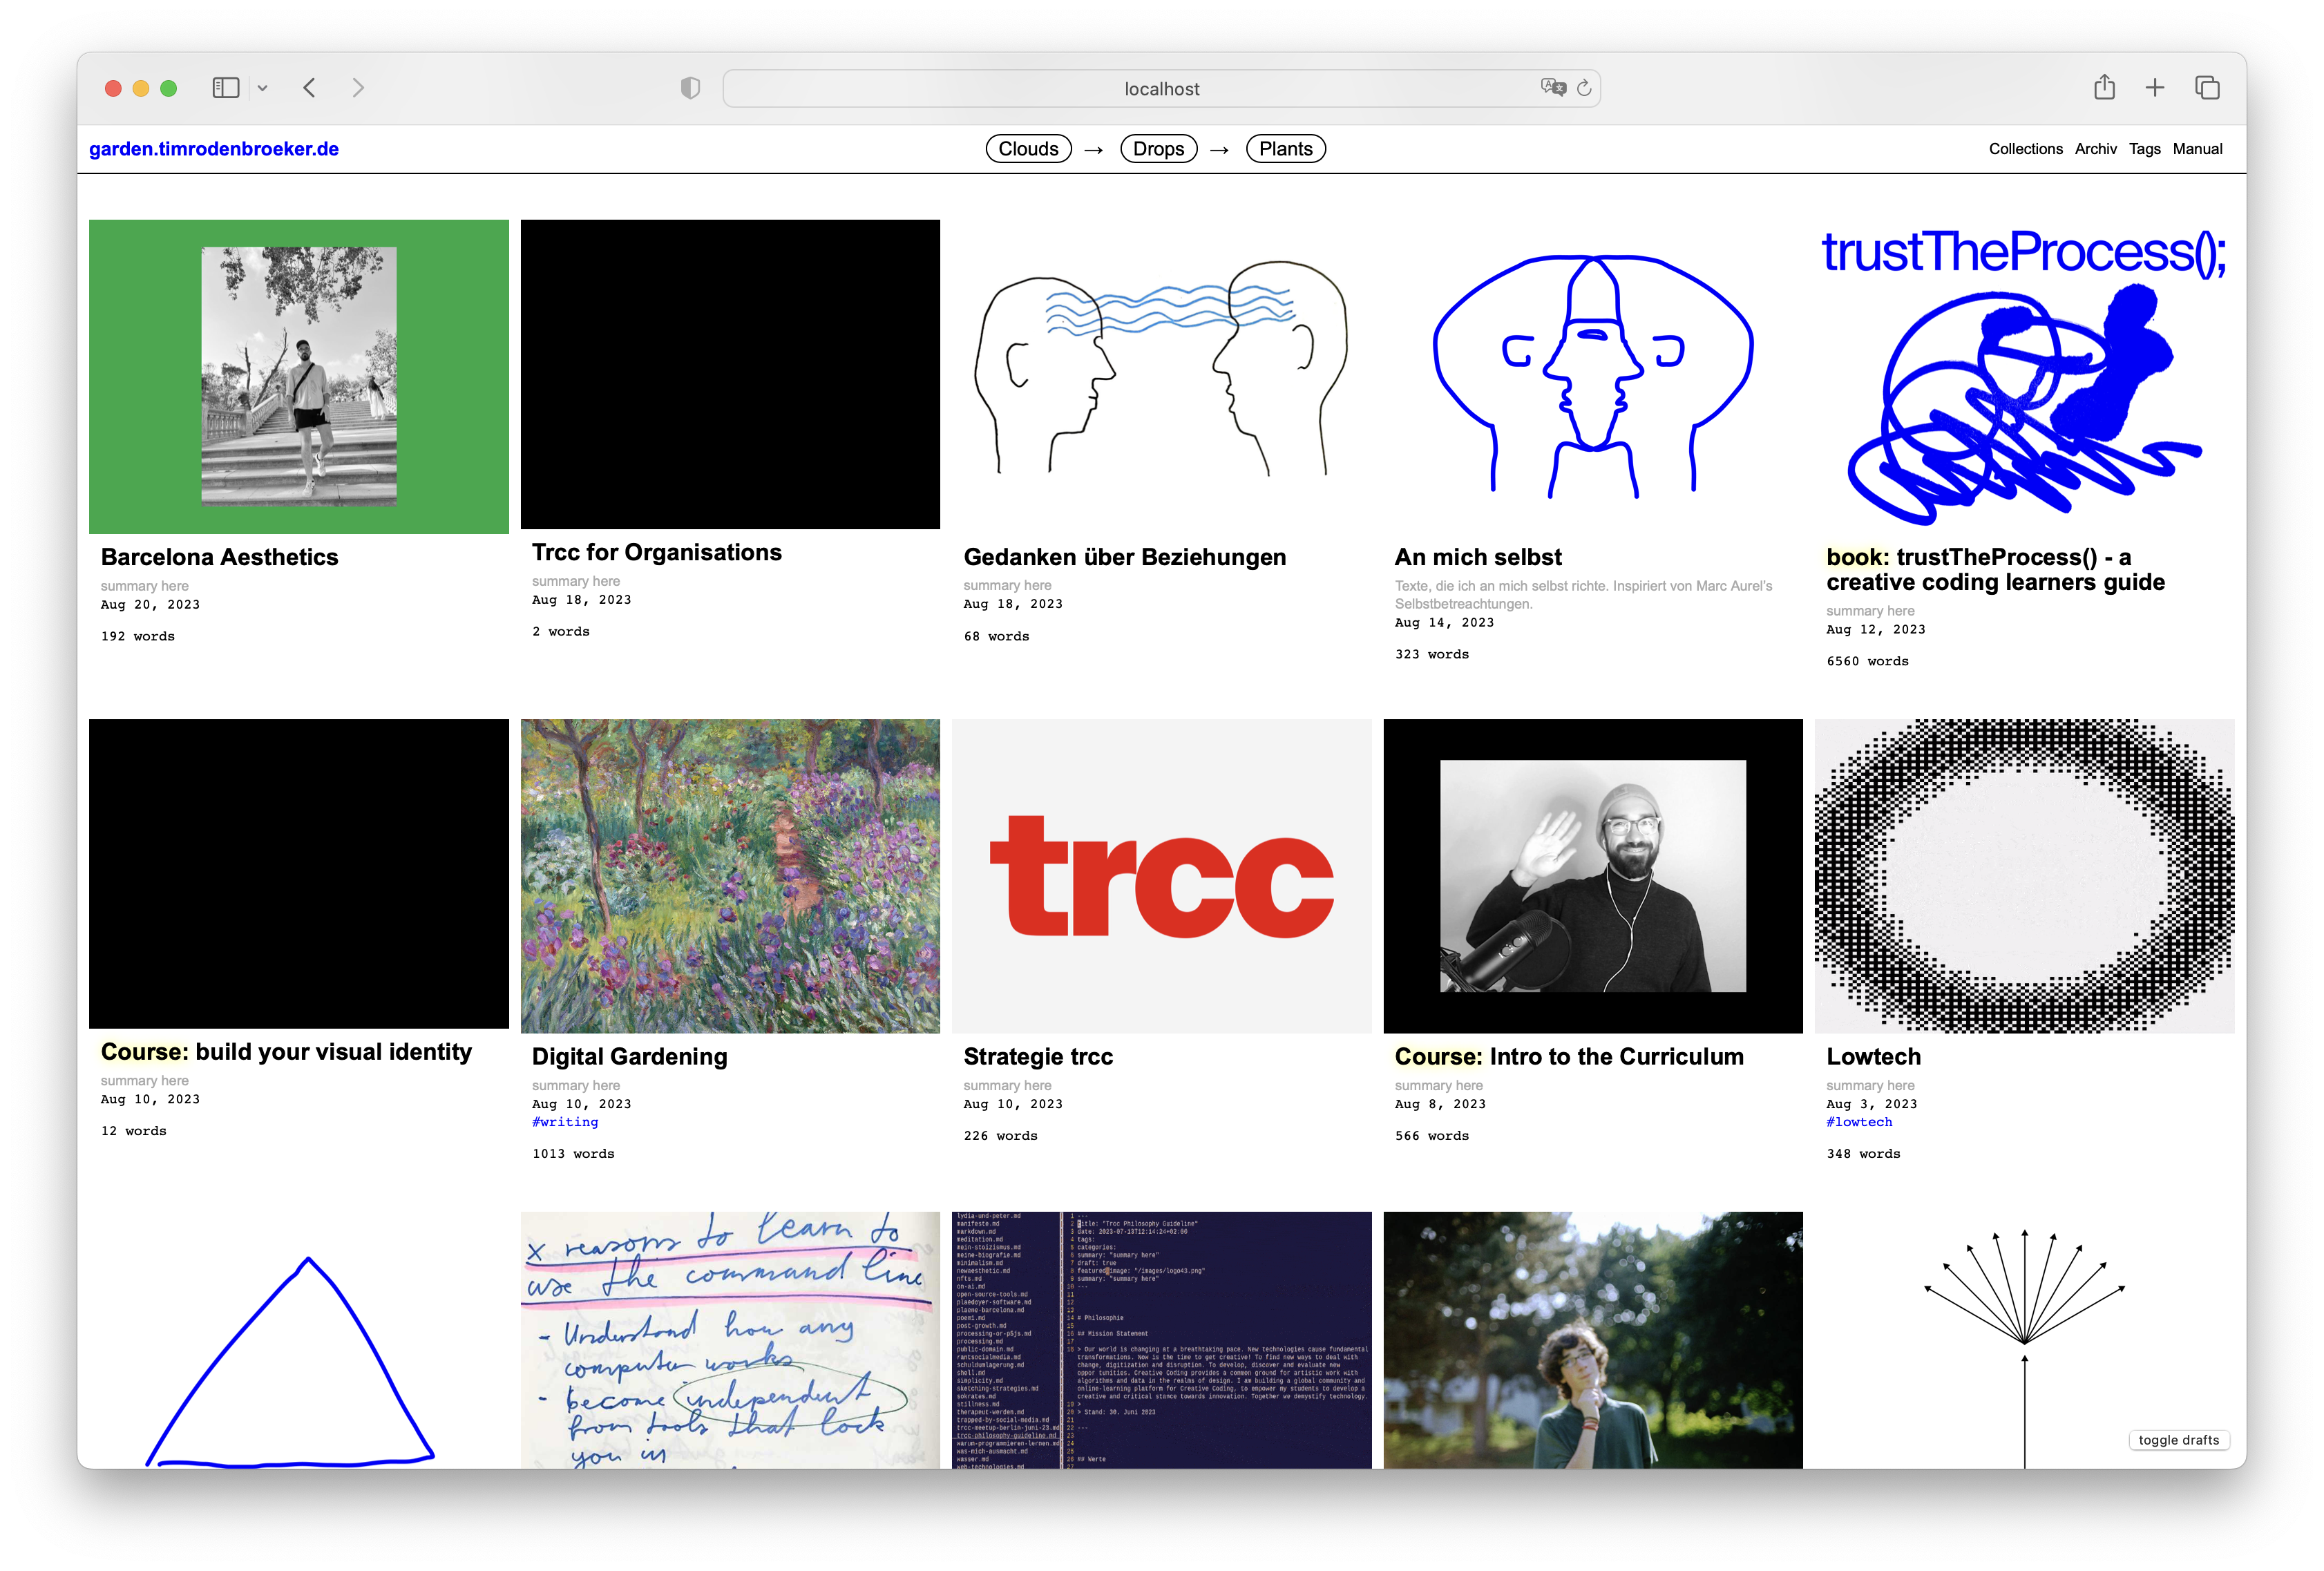
\includegraphics[width=8.33333in,height=\textheight]{images/dg1.png}

\caption{\label{fig-tim}Digital Garden by Tim Rodenböcker (Source:
\url{https://downgrade.timrodenbroeker.de/images/dg1.png})}

\end{figure}%

\begin{quote}
``I have now created such a file for all the books I have had in my
hands in the last few years. I write a note there when I find a thought
interesting while reading or listening to it. Drops are fragments that
are too small to represent an independent text. They are tiny stores of
information, paragraphs, but also lists and loose notes. Sometimes it's
just a headline'' (Rodenbröker, 2023).
\end{quote}

\section{Conclusion}\label{conclusion}

To conlude for today, digital gardens provide a dynamic and creative
framework for personal knowledge management, seamlessly blending
flexible idea cultivation with modern digital tools to enhance
individual learning and creativity.

\section*{References}\label{references}
\addcontentsline{toc}{section}{References}

\phantomsection\label{refs}
\begin{CSLReferences}{1}{0}
\vspace{1em}

\bibitem[\citeproctext]{ref-appleton2020Brief}
Appleton, M. (2020). \emph{A brief history \& ethos of the digital
garden: A newly revived philosophy for publishing personal knowledge on
the web}. \url{https://maggieappleton.com/garden-history}

\bibitem[\citeproctext]{ref-rodenbroker2023How}
Rodenbröker, T. (2023). \emph{How i built myself a digital garden}.
\url{https://downgrade.timrodenbroeker.de/posts/digital-garden/}

\end{CSLReferences}




\end{document}
